\FloatBarrier
\section{Stage 1: Signal characterisation and sampling}
\subsection{Measured spectrum, window and bandwidth}
\label{sec:r11}
I use the complete unmodified NPY record. Here $ F_0,L $ denote reference
rate/count and $ f_s,N $ transmission rate/count. The reference time and
finite-record power conventions give 
\begin{equation}
 t_n=\frac{n}{F_0},\quad n=0,\ldots,L-1,\qquad
 T=\frac L{F_0}=\RecordSeconds\,\mathrm{s}.
 \label{eq:time-grid}
\end{equation}
\begin{equation}
 \widehat P=\frac1L\sum_{n=0}^{L-1}x[n]^2=\SignalPower,
 \qquad x_{\mathrm{RMS}}=\sqrt{\widehat P}\simeq0.85440037.
 \label{eq:finite-power}
\end{equation}
The last timestamp is $(L-1)/F_0 $, not $ T $. Amplitudes/RMSE retain NPY
units; powers/MSE use their squares. The FFT computes the reference DFT
with an unscaled forward transform and $1/L $ inverse
(Appendix~\ref{app:dft}); it does not define a different transform
 \citep{cooley1965fft}.
Native spacing is $\BinSpacing $ Hz, with no padding. A real FFT displays
conjugate pairs once: interior amplitudes are doubled and divided by
the window sum, while DC/even Nyquist are not doubled
(Eq.~\eqref{eq:window-amplitude}). Power pairing doubles raw coefficient
powers once, not an already doubled amplitude squared.

\paragraph{Choose the window by measured comparison.}
I retain the rectangular window and cross-check the symmetric Hann
of Eq.~\eqref{eq:hann}, following a controlled window comparison. Hann coherent gain is $\HannGain $; after correction,
the four amplitudes differ by at most $\HannDifference $ NPY units.
Coherence is supported by the phase-aware whole-record fit below and
all remaining rectangular bins being below $\OtherBinDb $ dB, not merely
by integer indices assigned to detected peaks:
\begin{equation}
 \begin{aligned}
 \phi_j&=\arg X[k_j],\qquad
 \widehat x_m[n]=\sum_j\widehat A[k_j]\cos(2\pi f_jn/F_0+\phi_j),\\
 e_{m,\mathrm{RMS}}&=\sqrt{\frac1L\sum_n(x[n]-\widehat x_m[n])^2}
 =\ResidualRms.
 \end{aligned}
 \label{eq:component-model}
\end{equation}

\begin{figure}[!htbp]
 \centering
 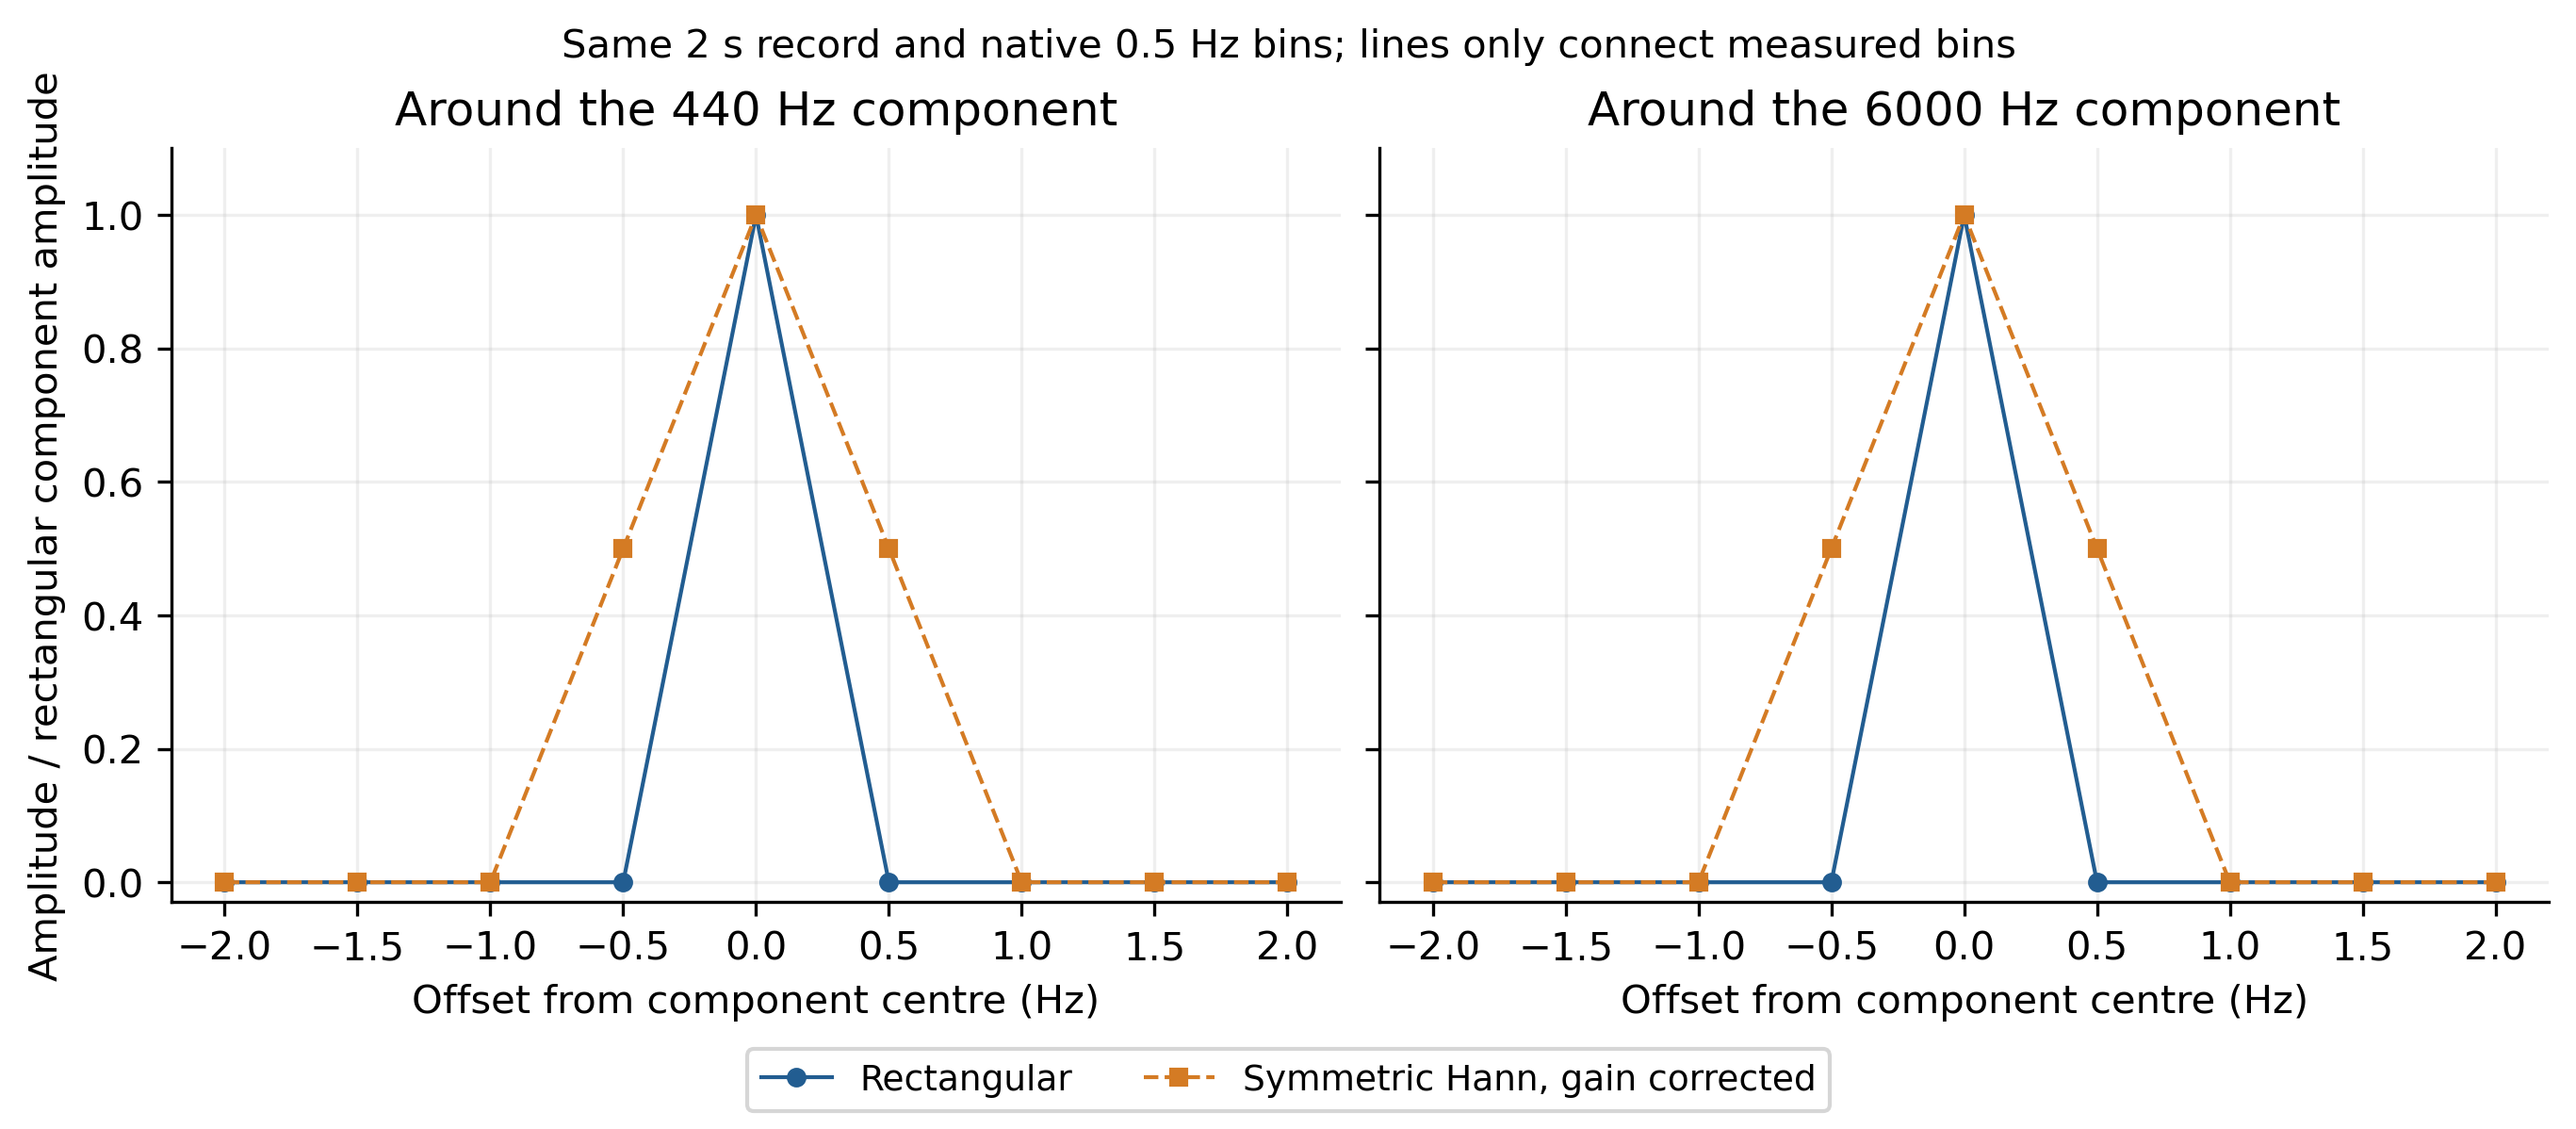
\includegraphics[width=.78\linewidth]{images/window_comparison.png}
 \caption{Same-record window comparison on native 0.5 Hz bins. Hann amplitudes are gain-corrected; adjacent skirts are not additional source tones.}
 \label{fig:window-check}
\end{figure}

The measured tones satisfy $ f_jT\in\mathbb Z $. Hann spreads them into
adjacent bins, including 6000.5 Hz; that bin is not a fifth source tone.
Rectangular therefore retains the narrow coherent peaks here; this choice
does not generalise to noncoherent records. Coherent-gain correction alone
does not remove off-bin or overlapping-tone bias \citep{harris1978windows}.

\paragraph{Define and test bandwidth rather than read a plot by eye.}
\begin{align}
 A_{\mathrm{ref}}&=\max_k\widehat A_R[k],\qquad
 D_w[k]=20\log_{10}\!\left(\frac{\widehat A_w[k]}{A_{\mathrm{ref}}}\right),
 \label{eq:relative-db}\\
 \mathcal K_\theta&=\{k:\ k\text{ is a local maximum and }
 \widehat A_w[k]\ge A_{\mathrm{ref}}10^{\theta/20}\},\qquad\theta=-60\,\mathrm{dB},
 \label{eq:component-detector}\\
 f_B&=\max_{k\in\mathcal K_\theta}f_k=\BandEdgeHz\,\mathrm{Hz}.
 \label{eq:band-edge}
\end{align}
Interior maxima use left-strict/right-nonstrict comparison, with endpoints
tested separately. The operational $-60 $ dB threshold is a project choice;
both windows retain the same four centres at $-40,-60,-80 $ dB. The weakest
tone is about $-20 $ dB. Table~\ref{tab:components} gives measured frequency,
amplitude and power; Figure~\ref{fig:sampling-summary} combines the
full spectrum with the resulting rate decision.

\begin{table}[tbp]
 \centering
 \caption{Measured source components from CSV, in unmodified NPY units. Relative dB uses the largest peak; powers use the paired-coefficient convention.}
 \label{tab:components}
 \begin{tabular}{rrrrr}
\toprule
Bin & Frequency (Hz) & Amplitude & Relative dB & Power (\%) \\
\midrule
880 & 440 & 1.0 & 0.000 & 68.4932 \\
2640 & 1320 & 0.6 & -4.437 & 24.6575 \\
4400 & 2200 & 0.3 & -10.458 & 6.1644 \\
12000 & 6000 & 0.1 & -20.000 & 0.6849 \\
\bottomrule
\end{tabular}

\end{table}

For the alternative cumulative-power definition,
\begin{equation}
 B_q=\min\left\{f_k:\frac{\sum_{i=0}^{k}P_i}{\sum_iP_i}\ge q\right\},
 \label{eq:energy-bandwidth}
\end{equation}
$ B_{0.99}=2200 $ Hz would discard the valid 6 kHz tone, which contributes
0.685 \% of power; $ B_{0.999}=6000 $ Hz retains it. I use the 6 kHz component
edge to preserve every identified tone. This is finite-record evidence,
not strict compact support of its time-truncated DTFT or an unknown
analogue source. Tone powers 0.5, 0.18, 0.045, 0.005 sum to 0.73.
Ten deterministic checks include DC/Nyquist/odd-length scaling, explicit
DFT sums, FFT agreement, inverse, Hann gain and Parseval. Relative
Parseval error is $\ParsevalError $ and maximum same-grid inverse error
is $\RoundTripError $; these checks are distinct from low-rate reconstruction.
